\documentclass[tikz, border=10pt]{standalone}
\usetikzlibrary{shapes.geometric, positioning, calc}

\begin{document}
	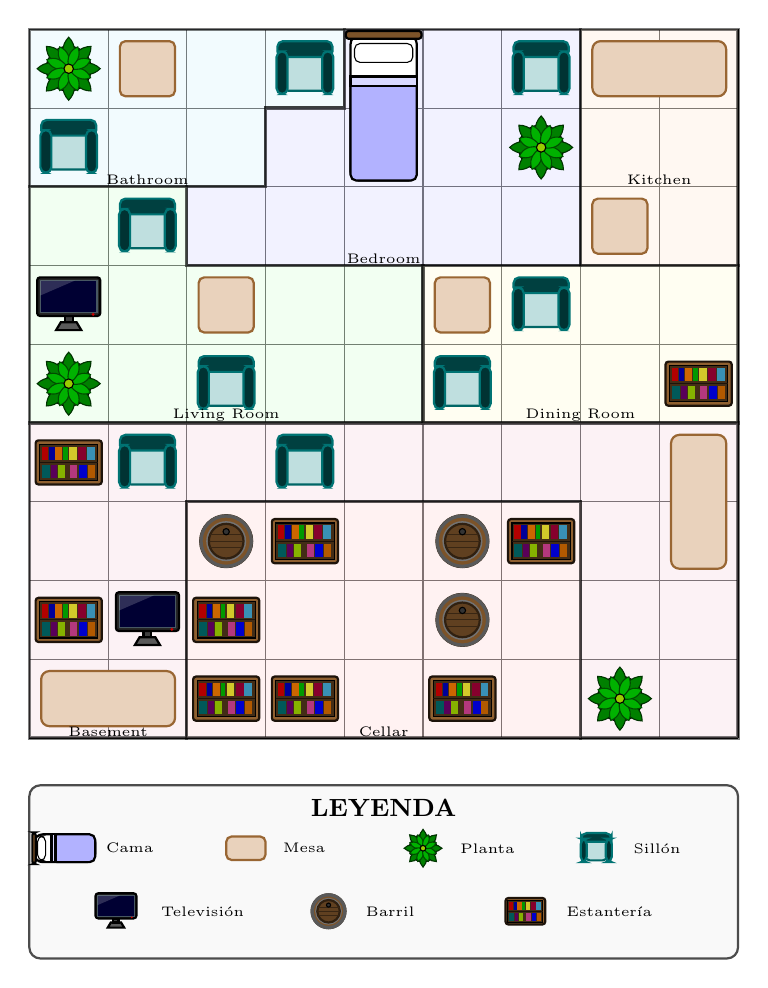
\begin{tikzpicture}
		
		% -------------------------------------------------------------
		% RED DE CELDAS (LÍNEAS SUAVES GRISES)
		% -------------------------------------------------------------
		\begin{scope}[black, thin]
			\foreach \x in {0.5, 1.5, ..., 9.5}
			\draw (\x, 0.5) -- (\x, -8.5);
			\foreach \y in {0.5, -0.5, ..., -8.5}
			\draw (0.5, \y) -- (9.5, \y);
		\end{scope}
		
		% -------------------------------------------------------------
		% DELIMITACIÓN / RELLENO DE ZONAS
		% -------------------------------------------------------------
		
		% Baño: (1,1)-(1,4), (2,1)-(2,3)
		\draw[very thick, fill=cyan!10, opacity=0.5] 
		(0.5, 0.5) -- (4.5, 0.5) -- (4.5, -0.5) -- (3.5, -0.5) -- 
		(3.5, -1.5) -- (0.5, -1.5) -- cycle;
		
		% Dormitorio principal: (1,5)-(1,7), (2,4)-(2,7), (3,3)-(3,7)
		\draw[very thick, fill=blue!10, opacity=0.5] 
		(4.5, 0.5) -- (7.5, 0.5) -- (7.5, -2.5) -- (2.5, -2.5) -- 
		(2.5, -1.5) -- (3.5, -1.5) -- (3.5, -0.5) -- (4.5, -0.5) -- cycle;
		
		% Cocina: (1,8)-(3,9)
		\draw[very thick, fill=orange!10, opacity=0.5] 
		(7.5, 0.5) -- (9.5, 0.5) -- (9.5, -2.5) -- (7.5, -2.5) -- cycle;
		
		% Salón: (3,1)-(3,2), (4,1)-(5,5)
		\draw[very thick, fill=green!10, opacity=0.5] 
		(0.5, -1.5) -- (2.5, -1.5) -- (2.5, -2.5) -- (5.5, -2.5) -- 
		(5.5, -4.5) -- (0.5, -4.5) -- cycle;
		
		% Comedor: (4,6)-(5,9)
		\draw[very thick, fill=yellow!10, opacity=0.5] 
		(5.5, -2.5) -- (9.5, -2.5) -- (9.5, -4.5) -- (5.5, -4.5) -- cycle;
		
		% Sótano: Fila 6 (1-9) + Patas 7-9 (cols 1-2 y 8-9)
		\draw[very thick, fill=purple!10, opacity=0.5] 
		(0.5, -4.5) -- (9.5, -4.5) -- (9.5, -8.5) -- (7.5, -8.5) -- 
		(7.5, -5.5) -- (2.5, -5.5) -- (2.5, -8.5) -- (0.5, -8.5) -- cycle;
		
		% Bodega: (7,3)-(9,7)
		\draw[very thick, fill=red!10, opacity=0.5] 
		(2.5, -5.5) -- (7.5, -5.5) -- (7.5, -8.5) -- (2.5, -8.5) -- cycle;
		
		
		% -------------------------------------------------------------
		% MOBILIARIO: CAMA (Celdas 1,5 y 2,5)
		% -------------------------------------------------------------
		\tikzset{
			pics/cama/.style={
				code={
					% Colchón base / Sábana
					\draw[thick, fill=white, rounded corners=3pt] (-0.42, -0.92) rectangle (0.42, 0.92);
					% Cabecero
					\draw[thick, fill=brown!65!black, rounded corners=1pt] (-0.48, 0.88) rectangle (0.48, 0.98);
					% Manta / Edredón (extendida hasta 0.40)
					\draw[thick, fill=blue!30!white, rounded corners=2pt] (-0.42, -0.92) rectangle (0.42, 0.40);
					% Dobladillo de la manta (en el borde superior de la manta)
					\draw[thick, fill=blue!15!white] (-0.42, 0.28) rectangle (0.42, 0.40);
					% Almohadas (desplazadas cerca del cabecero: 0.58 a 0.82)
					\draw[thin, fill=white, rounded corners=2pt] (-0.37, 0.58) rectangle (0.37, 0.82);
				}
			}
		}
		
		\path (5, -0.5) pic {cama};  % Ubicación en el Dormitorio Principal
		
		% -------------------------------------------------------------
		% MOBILIARIO: MESAS
		% -------------------------------------------------------------
		\tikzset{
			mesa style/.style={thick, fill=brown!35!white, draw=brown!80!black}
		}
		
		% Mesa 1: Celda (1,2)
		\draw[mesa style, rounded corners=2pt] (1.65, -0.35) rectangle (2.35, 0.35);
		
		% Mesa 2: Celdas (1,8) y (1,9)
		\draw[mesa style, rounded corners=3pt] (7.65, -0.35) rectangle (9.35, 0.35);
		
		% Mesa 3: Celda (3,8)
		\draw[mesa style, rounded corners=2pt] (7.65, -2.35) rectangle (8.35, -1.65);
		
		% Mesa 4: Celda (4,3)
		\draw[mesa style, rounded corners=2pt] (2.65, -3.35) rectangle (3.35, -2.65);
		
		% Mesa 5: Celda (4,6)
		\draw[mesa style, rounded corners=2pt] (5.65, -3.35) rectangle (6.35, -2.65);
		
		% Mesa 6: Celdas (6,9) y (7,9)
		\draw[mesa style, rounded corners=3pt] (8.65, -6.35) rectangle (9.35, -4.65);
		
		% Mesa 7: Celdas (9,1) y (9,2)
		\draw[mesa style, rounded corners=3pt] (0.65, -8.35) rectangle (2.35, -7.65);
		
		
		% -------------------------------------------------------------
		% MOBILIARIO: PLANTAS
		% -------------------------------------------------------------
		\tikzset{
			pics/planta/.style={
				code={
					\draw[thick, fill=brown!60!black] (0,0) circle (0.28);
					\draw[fill=brown!30!black] (0,0) circle (0.22);
					\foreach \a in {0, 45, ..., 315} {
						\draw[fill=green!50!black, draw=green!20!black, thin] (0,0) [rotate=\a] 
						.. controls (0.1,0.15) and (0.1,0.3) .. (0,0.4) 
						.. controls (-0.1,0.3) and (-0.1,0.15) .. (0,0);
					}
					\foreach \a in {22.5, 67.5, ..., 337.5} {
						\draw[fill=green!70!black, draw=green!30!black, thin] (0,0) [rotate=\a] 
						.. controls (0.08,0.12) and (0.08,0.22) .. (0,0.3) 
						.. controls (-0.08,0.22) and (-0.08,0.12) .. (0,0);
					}
					\draw[fill=lime!80!black] (0,0) circle (0.06);
				}
			}
		}
		
		\path (1,0) pic {planta};   % Celda (1,1)
		\path (7,-1) pic {planta};  % Celda (2,7)
		\path (1,-4) pic {planta};  % Celda (5,1)
		\path (8,-8) pic {planta};  % Celda (9,8)
		
		
		% -------------------------------------------------------------
		% MOBILIARIO: SILLONES
		% -------------------------------------------------------------
		\tikzset{
			pics/sillon/.style={
				code={
					% Asiento / Cojín
					\draw[thick, fill=teal!25!white, draw=teal!80!black, rounded corners=2pt] (-0.28, -0.28) rectangle (0.28, 0.28);
					% Respaldo
					\draw[thick, fill=teal!50!black, draw=teal!90!black, rounded corners=2pt] (-0.35, 0.15) rectangle (0.35, 0.35);
					% Reposabrazos
					\draw[thick, fill=teal!40!black, draw=teal!90!black, rounded corners=2pt] (-0.36, -0.32) rectangle (-0.22, 0.22);
					\draw[thick, fill=teal!40!black, draw=teal!90!black, rounded corners=2pt] (0.22, -0.32) rectangle (0.36, 0.22);
				}
			}
		}
		
		\path (4,0)  pic {sillon};  % Celda (1,4)
		\path (7,0)  pic {sillon};  % Celda (1,7)
		\path (1,-1) pic {sillon};  % Celda (2,1)
		\path (2,-2) pic {sillon};  % Celda (3,2)
		\path (7,-3) pic {sillon};  % Celda (4,7)
		\path (3,-4) pic {sillon};  % Celda (5,3)
		\path (6,-4) pic {sillon};  % Celda (5,6)
		\path (2,-5) pic {sillon};  % Celda (6,2)
		\path (4,-5) pic {sillon};  % Celda (6,4)
		
		
		% -------------------------------------------------------------
		% MOBILIARIO: TELEVISIONES (VISTA FRONTAL)
		% -------------------------------------------------------------
		\tikzset{
			pics/tv/.style={
				code={
					% Peana / Base del soporte
					\draw[thick, fill=gray!70!black] (-0.16, -0.32) -- (0.16, -0.32) -- (0.10, -0.22) -- (-0.10, -0.22) -- cycle;
					% Cuello del soporte
					\draw[thick, fill=gray!50!black] (-0.05, -0.22) rectangle (0.05, -0.14);
					% Marco exterior de la TV
					\draw[thick, fill=black!85, rounded corners=1pt] (-0.40, -0.14) rectangle (0.40, 0.35);
					% Pantalla
					\draw[fill=blue!20!black, draw=cyan!30!black] (-0.36, -0.10) rectangle (0.36, 0.31);
					% Reflejo en la pantalla
					\fill[white, opacity=0.18] (-0.36, 0.12) -- (0.08, 0.31) -- (-0.36, 0.31) -- cycle;
					% Luz LED de encendido
					\fill[red!80!black] (0.31, -0.12) circle (0.02);
				}
			}
		}
		
		\path (1,-3) pic {tv};  % Celda (4,1) - Salón
		\path (2,-7) pic {tv};  % Celda (8,2) - Sótano
		
		
		% -------------------------------------------------------------
		% MOBILIARIO: BARRILES DE MADERA
		% -------------------------------------------------------------
		\tikzset{
			pics/barril/.style={
				code={
					% Cuerpo de madera exterior
					\draw[thick, fill=brown!65!black, draw=brown!30!black] (0,0) circle (0.33);
					% Aros metálicos de refuerzo
					\draw[very thick, black!65] (0,0) circle (0.32);
					\draw[thick, black!55] (0,0) circle (0.24);
					% Tapa superior de madera
					\draw[thick, fill=brown!50!black, draw=brown!25!black] (0,0) circle (0.22);
					% Tablas de la tapa
					\draw[brown!30!black, thin] (-0.20, 0.08) -- (0.20, 0.08);
					\draw[brown!30!black, thin] (-0.22, 0.00) -- (0.22, 0.00);
					\draw[brown!30!black, thin] (-0.20, -0.08) -- (0.20, -0.08);
					% Tapón central
					\draw[fill=black!80] (0, 0.12) circle (0.04);
				}
			}
		}
		
		\path (3,-6) pic {barril};  % Celda (7,3) - Bodega
		\path (6,-6) pic {barril};  % Celda (7,6) - Bodega
		\path (6,-7) pic {barril};  % Celda (8,6) - Bodega
		
		
		% -------------------------------------------------------------
		% MOBILIARIO: ESTANTERÍAS / LIBRERÍAS
		% -------------------------------------------------------------
		\tikzset{
			pics/estanteria/.style={
				code={
					% Estructura/Marco de madera
					\draw[thick, fill=brown!75!black, draw=brown!15!black, rounded corners=1pt] (-0.42, -0.28) rectangle (0.42, 0.28);
					% Fondo interno
					\draw[fill=brown!35!black] (-0.37, -0.23) rectangle (0.37, 0.23);
					% Balda divisoria horizontal
					\draw[brown!15!black, thin] (-0.37, 0) -- (0.37, 0);
					% Libros en la balda superior
					\fill[red!70!black]    (-0.34,  0.03) rectangle (-0.26,  0.20);
					\fill[blue!60!black]   (-0.25,  0.03) rectangle (-0.18,  0.20);
					\fill[orange!80!black] (-0.17,  0.03) rectangle (-0.08,  0.20);
					\fill[green!60!black]  (-0.07,  0.03) rectangle (-0.01,  0.20);
					\fill[yellow!80!black] ( 0.01,  0.03) rectangle ( 0.10,  0.20);
					\fill[purple!70!black] ( 0.12,  0.03) rectangle ( 0.22,  0.20);
					\fill[cyan!70!black]   ( 0.23,  0.03) rectangle ( 0.33,  0.20);
					% Libros en la balda inferior
					\fill[teal!70!black]   (-0.34, -0.20) rectangle (-0.24, -0.03);
					\fill[violet!70!black] (-0.23, -0.20) rectangle (-0.15, -0.03);
					\fill[lime!70!black]   (-0.14, -0.20) rectangle (-0.05, -0.03);
					\fill[magenta!70!black]( 0.02, -0.20) rectangle ( 0.11, -0.03);
					\fill[blue!80!black]   ( 0.13, -0.20) rectangle ( 0.23, -0.03);
					\fill[orange!70!black] ( 0.24, -0.20) rectangle ( 0.33, -0.03);
				}
			}
		}
		
		% Posiciones solicitadas (x = columna, y = -(fila-1))
		\path (9,-4) pic {estanteria};  % Celda (5,9) - Comedor
		\path (1,-5) pic {estanteria};  % Celda (6,1) - Sótano
		\path (4,-6) pic {estanteria};  % Celda (7,4) - Bodega
		\path (7,-6) pic {estanteria};  % Celda (7,7) - Bodega
		\path (1,-7) pic {estanteria};  % Celda (8,1) - Sótano
		\path (3,-7) pic {estanteria};  % Celda (8,3) - Bodega
		\path (3,-8) pic {estanteria};  % Celda (9,3) - Bodega
		\path (4,-8) pic {estanteria};  % Celda (9,4) - Bodega
		\path (6,-8) pic {estanteria};  % Celda (9,6) - Bodega
		
		
		% -------------------------------------------------------------
		% ETIQUETAS EN TAMAÑO TINY (Parte inferior de cada zona)
		% -------------------------------------------------------------
		
		% Baño (Centrado en la fila 2, cols 1-3)
		\node[font=\tiny, anchor=south] at (2, -1.6) {Bathroom};
		
		% Dormitorio principal (Centrado en la fila 3, col 5)
		\node[font=\tiny, anchor=south] at (5, -2.6) {Bedroom};
		
		% Cocina (Centrado en la fila 2, cols 8-9)
		\node[font=\tiny, anchor=south] at (8.5, -1.6) {Kitchen};
		
		% Salón (Centrado en la fila 5, col 3)
		\node[font=\tiny, anchor=south] at (3, -4.6) {Living Room};
		
		% Comedor (Centrado en la fila 5, cols 6-9)
		\node[font=\tiny, anchor=south] at (7.5, -4.6) {Dining Room};
		
		% Sótano (Centrado en la parte inferior izquierda: fila 9, cols 1-2)
		\node[font=\tiny, anchor=south] at (1.5, -8.6) {Basement};
		
		% Bodega (Centrado en la fila 9, col 5)
		\node[font=\tiny, anchor=south] at (5, -8.6) {Cellar};
		
		
		% -------------------------------------------------------------
		% LEYENDA DE MOBILIARIO
		% -------------------------------------------------------------
		% Marco contenedor de la leyenda
		\draw[thick, fill=gray!5, draw=black!70, rounded corners=4pt] (0.5, -9.1) rectangle (9.5, -11.3);
		\node[font=\small\bfseries, anchor=north] at (5, -9.15) {LEYENDA};
		
		% Fila 1 de la leyenda (y = -9.9)
		% Cama
		\path (0.95, -9.9) pic[rotate=90, scale=0.42, transform shape] {cama};
		\node[font=\tiny, anchor=west] at (1.35, -9.9) {Cama};
		
		% Mesa
		\draw[mesa style, rounded corners=2pt] (3.0, -10.05) rectangle (3.5, -9.75);
		\node[font=\tiny, anchor=west] at (3.6, -9.9) {Mesa};
		
		% Planta
		\path (5.5, -9.9) pic[scale=0.6] {planta};
		\node[font=\tiny, anchor=west] at (5.85, -9.9) {Planta};
		
		% Sillón (utiliza el pic del tablero con 'transform shape' para mantener proporciones)
		\path (7.7, -9.9) pic[scale=0.55, transform shape] {sillon};
		\node[font=\tiny, anchor=west] at (8.05, -9.9) {Sillón};
		
		% Fila 2 de la leyenda (y = -10.7)
		% Televisión
		\path (1.6, -10.7) pic[scale=0.65] {tv};
		\node[font=\tiny, anchor=west] at (2.05, -10.7) {Televisión};
		
		% Barril
		\path (4.3, -10.7) pic[scale=0.65] {barril};
		\node[font=\tiny, anchor=west] at (4.65, -10.7) {Barril};
		
		% Estantería
		\path (6.8, -10.7) pic[scale=0.6] {estanteria};
		\node[font=\tiny, anchor=west] at (7.2, -10.7) {Estantería};
		
	\end{tikzpicture}
\end{document}